\Chapter{Monte-Carlo Simulations for PROSPECT}
\label{Ch6}

In PROSPECT's reactor neutrino measurement, Monte-Carlo simulation (MC) is necessary to 
\begin{itemize}
	\item Test detector configurations during R\&D
	\item Characterize detector performance
	\item Study detector energy response to a variety of particles
	\item Determine systematic uncertainties of detector geometry and light response
	\item Generate spectrum models and toys for parameter searches and sensitivity studies
\end{itemize}
PROSPECT-G4 (PG4) is the PROSPECT customized MC simulation package programmed based on the Geant-4~\cite{bib:geant4} toolkit.
This simulation package allows users to adjust detector geometries and material properties to provide important information guiding detector design. 
PG4 was developed with prototype detectors; and was used to demonstrate the simulation's reproduction of calibration data.
Because of limitations in computing resources and time, PG4 contains necessary simplifications in its description of PROSPECT's detector geometry and particle interactions.
Adjusting PG4's simulation of detector geometry, particle generation functions, and energy response is one of the essential parts in my thesis research.

\Section{Geometrical Simulation}

PROSPECT detector configurations are simulated in PG4. 
The simulated structures include $^6$LiLS, the optical grid, PMT modules, containers, and shielding.
Although most of the materials utilized in the PROSPECT AD are saved in Geant4 material databases with their chemical components and densities, $^6$LiLS is customized in PG4 by characterizing the density, chemical components, and doping percentage of the scintillator.
The simulated $^6$LiLS is composed of 0.9781~g/cm$^3$ density EJ-309, which is composed of 84.14\% C, 9.52\% H, and 6.34\% O by weight.
Additional water and LiCl solution was added with the concentration easily adjustable in simulation.
The reflectances of the optical grid separators are set based on direct optical measurements described in Chapter~\ref{Ch4}.

Some approximations was made to simplify the programming and running of PG4.
The DAQ cables and systems are not included in the simulation because they do not contribute dead volume to the active detector volume.
For simplicity of programming, the separator pinching tabs of PLA rods are continuous from end to end along each cell.
The separator materials consist of only FEP films, and carbon fibers, as the density and chemical components of other laminated materials are not known.

For the radioactive calibration system, only calibration source capsules are simulated in PG4; the source driving components have minimal affect on dead volume in the detector. 
The source capsule materials and dimensions are programmed according to the actual design.

The on-site shielding wall and the detector shielding walls are also simulated based on the designed material and dimensions.

\Section{Particle Generation and Interaction Simulations}

Because of neutrinos' low IBD cross-section, direct neutrino simulation is not realistic in PG4. 
Instead, IBD produced positrons and neutrons are generated to mimic the IBD interaction in the detector. 
In PG4 simulation, each IBD event contains a positron-neutron pair generated from the same vertex with their sum of energy equal to a user defined neutrino energy plus a rest proton energy (the IBD total energy).
The IBD total energy and vertex position can be adjusted for different analysis purposes, including model generation, detector response studies and uncertainty calculations.
In the special case of simulating the reactor neutrinos generated from HFIR, IBD total energies are generated based on the Huber model of the reactor neutrino spectrum~\cite{bib:huber}.
As the reactor location is approximately 45$^\circ$ below the PROSPECT detector, the angular distribution of the IBD products is implemented as shown in Figure~\ref{fig:IBDangle}.

\begin{figure}[h!]
    \centering
    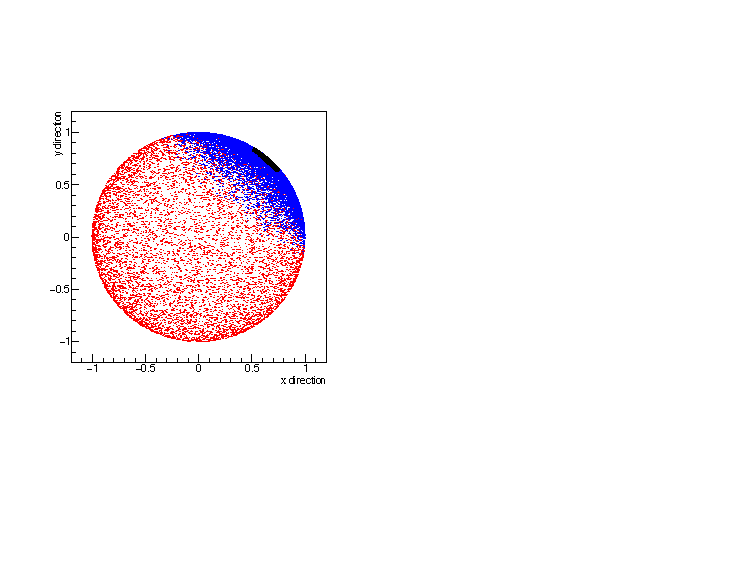
\includegraphics[width=0.7\textwidth]{Figures/IBDKinematics.pdf}
	\caption[The simulated IBD products angular distribution]{
    The simulated IBD products' angular distributions, with red dots representing positrons and blue dots representing neutrons.}
    \label{fig:IBDangle}
\end{figure}

Radioactive sources utilized in calibration are simulated in PG4 with custom built particle generators. 
The gammas and electrons of the calibration sources are generated from user defined vertexes with energies extracted from the energy levels and transition probabilities saved in the ENSDF database~\cite{bib:ENSDF}. 
For the $^{252}$Cf spontaneous fission neutron source, the emitted neutrons and gammas from its fission reaction are simulated instead of directly simulating the fission process. 

The cosmic ray background is simulated with the external cosmic ray shower generator CRY~\cite{bib:CRY}.

\Section{Truth-level Simulation}

Identification of particle type (PID) of PG4 is consistent with Geant4, which uses PDGID~\cite{bib:PDG} of particles.
In the case of neutron capture events, the $A$ and $Z$ values of the neutron capturing atoms are recorded.

Particle energy depositions and positions in the detector are tracked with the \texttt{G4Track} and \texttt{G4Step} objects, as illustrated in Figure~\ref{fig:g4step}.
\texttt{G4Track} is a snapshot of a particle.
Every two points in \texttt{G4Track} are connected by \texttt{G4Step}.
Every two steps are separated by 1) a particle interaction, 2) particle traversal through the boundary of two geometrical volumes in Geant4, 3) a particle traveled the maximum length of each step, 4) a particle stops or exits the simulation world volume.
\texttt{G4Track} saves the particle's PID, energy, and position information.
\texttt{G4Step} saves the particle's energy loss from the beginning to the end of a step.
Therefore, a particle's energy deposition in each segment of the PROSPECT AD can be saved by summing the the energy deposits in all steps in a segment. 
Each \texttt{G4Step}'s maximum length is set by user.
The step size is independent of particle energy and current medium.
As a result, the $dE/dx$ calculated in each step does not precisely reflect actual material stopping power.
\begin{figure}[h!]
    \centering
    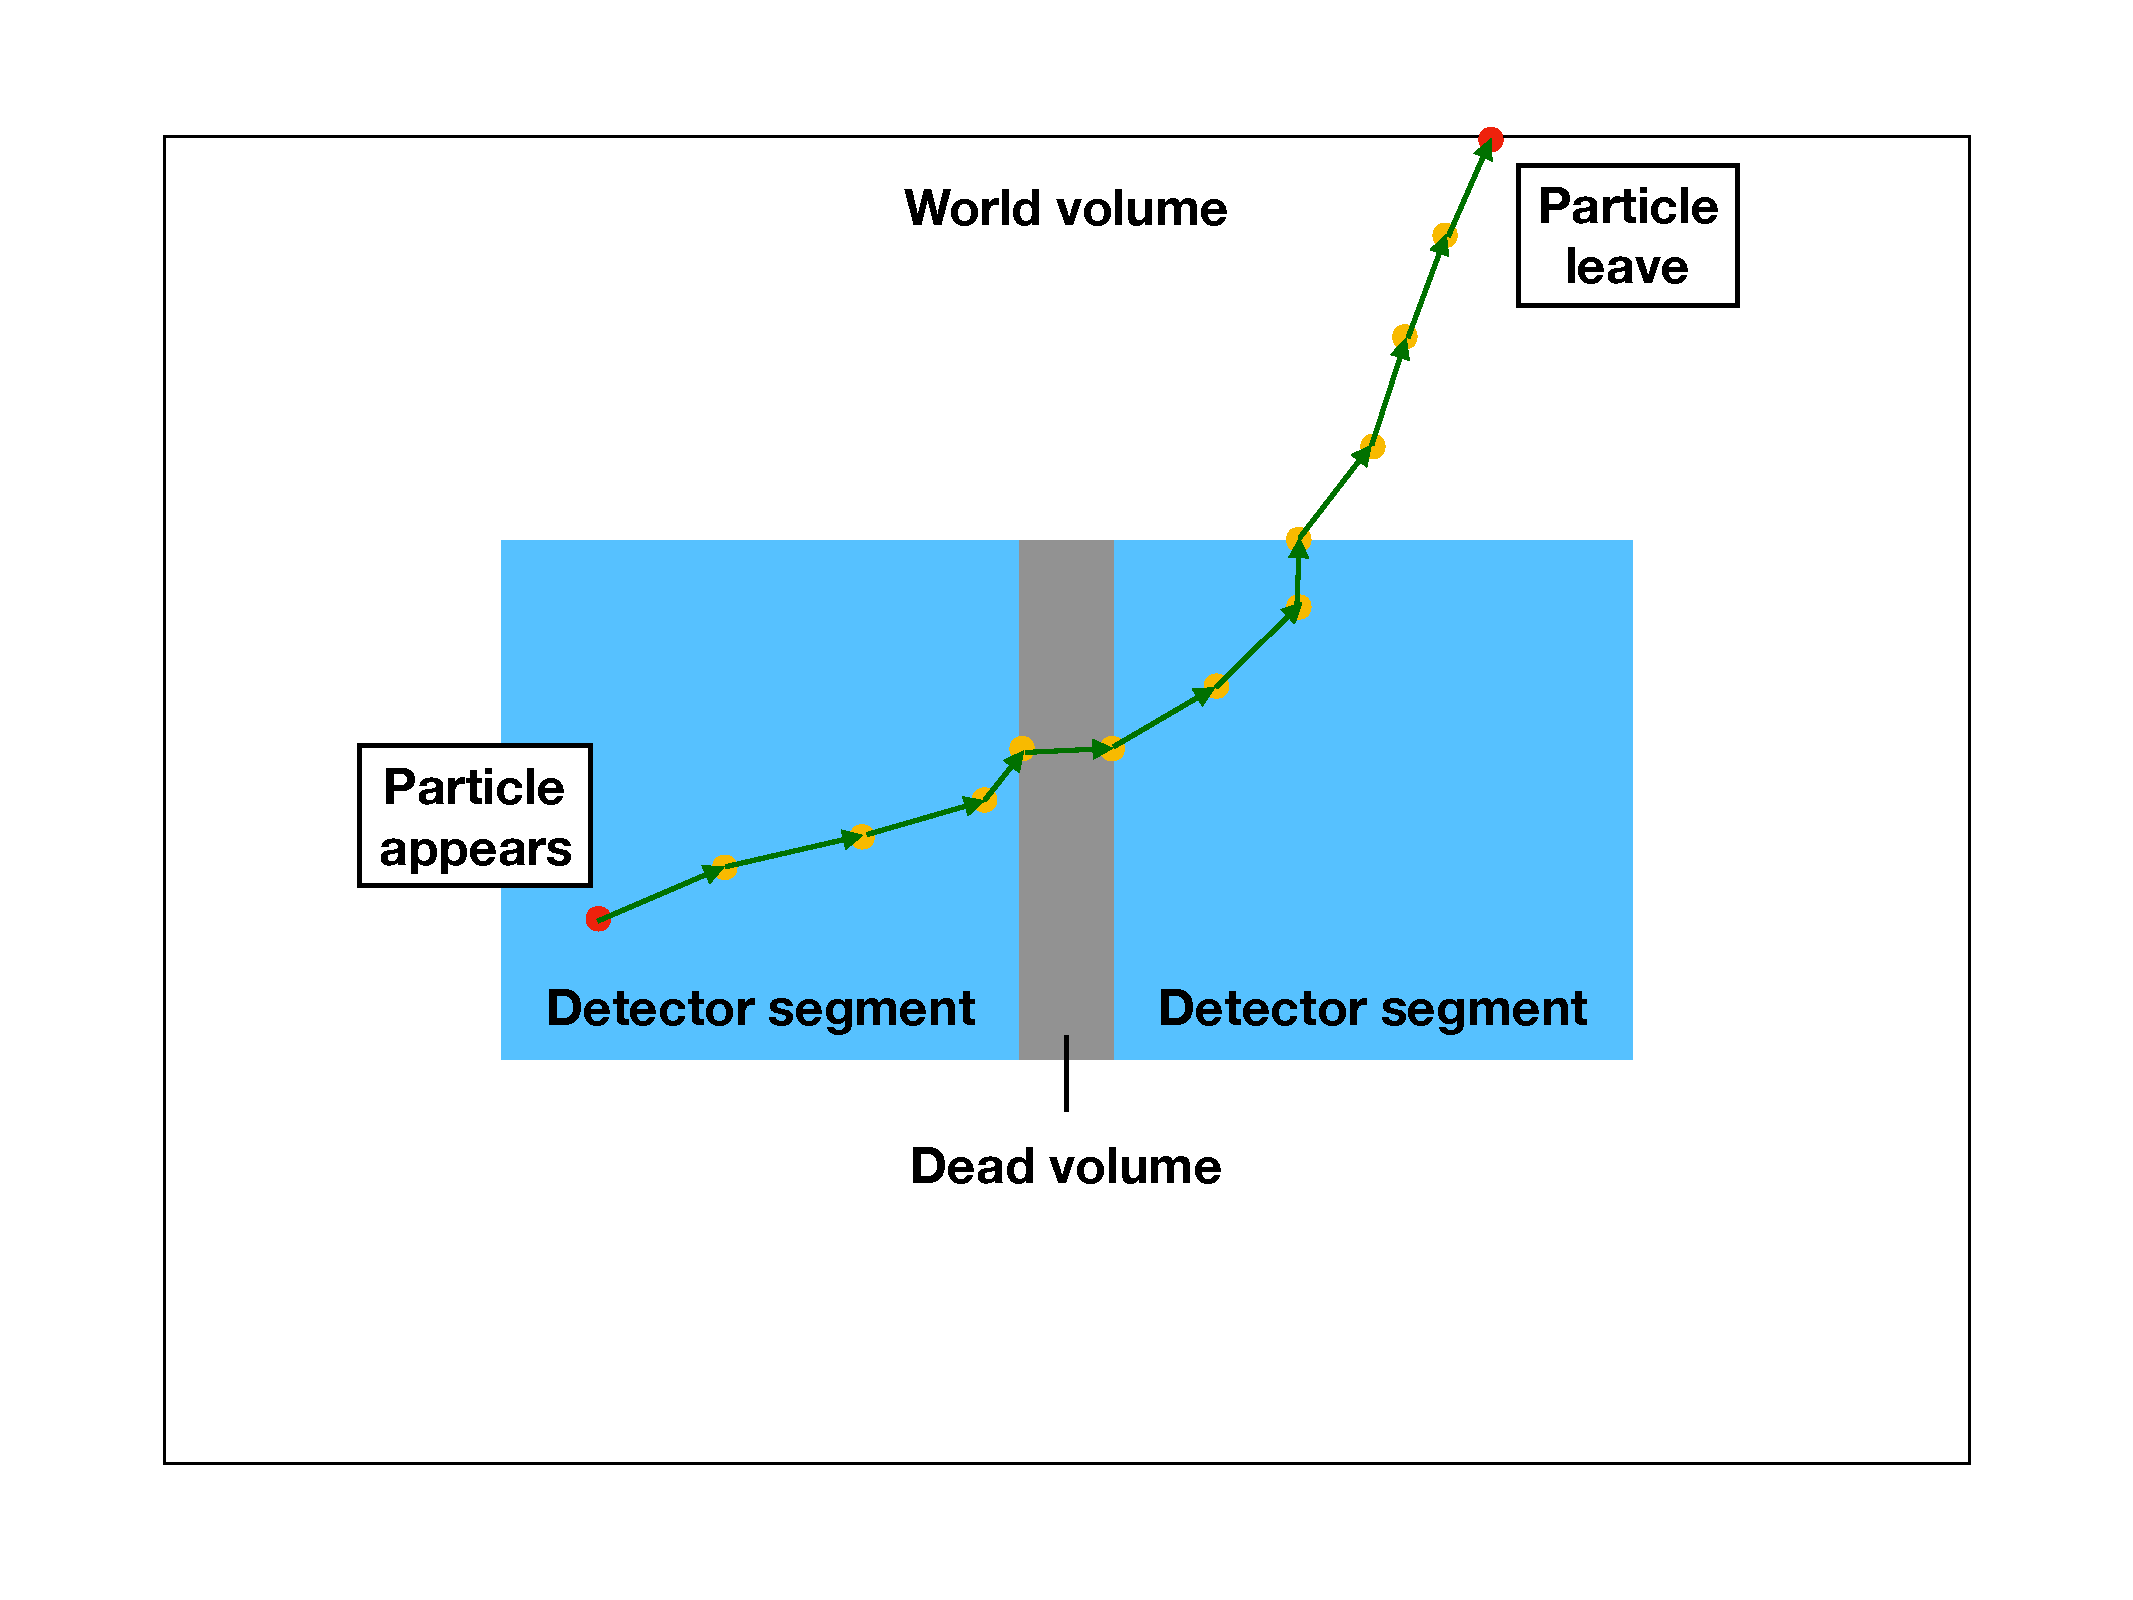
\includegraphics[width=0.8\textwidth]{Figures/G4Step.pdf}
	\caption[Illustration of PG4 event tracking]{
    An illustration of PG4 event tracking, where an arbitrary is recorded. 
    The yellow dots and the arrows connecting among them represent \texttt{G4Track}s and \texttt{G4Step}s.
    }
    \label{fig:g4step}
\end{figure}

PG4's ability to track a particle's energy loss step-by-step enables simulation of nonlinear detector response. 
In Chapter~\ref{Ch5}, the Birks' quenching function is determined as 
\begin{equation}
\frac{dL}{dx} = \frac{S\frac{dE}{dx}}{1+k_{B1}\frac{dE}{dx} + k_{B2}(\frac{dE}{dx})^2}.
\label{eq:birkslaw}
\end{equation}
Using the $dE/dx$ calculated by each step, the quenched light yield can be effectively expressed as the reduction of energy deposition 
\begin{equation}
   \frac{dE_{quench}}{dx} = \frac{\frac{dE}{dx}}{1+k_{B1}\frac{dE}{dx}+k_{B2}(\frac{dE}{dx})^2}.
\end{equation}
Hence, the quenched energy of a particle is
\begin{equation}
   E_{quench} = \sum_{i}^{steps}\frac{\frac{dE_i}{dx}}{1+k_{B1}\frac{dE_i}{dx}+k_{B2}(\frac{dE_i}{dx})^2}, 
   \label{eq:birksMC}
\end{equation}
where $k_{B1}$ and $k_{B2}$ are effective Birks' constants, since the $dE/dx$ calculated in each \texttt{G4Step} differs from actual material stopping power.
PG4's simulation of Birks' quenching is a unique approach in particle detector simulation.
It allows the user to adjust the detector's nonlinear response by changing the quenching factors ($k_{B1}$ and $k_{B2}$ ) of the simulated detector.
This is a necessary simulation feature because the event reconstruction for the segmented PROSPECT AD is complicated, as discussed in Chapter~\ref{Ch8}.

Cherenkov radiation can also be simplified using the energy loss and speed of particles calculated by PG4.
Because of limited computing resources, optical photon simulation for high energy interactions is unrealistic.
As discussed in Chapter~\ref{Ch5}, the number of photons generated as Cherenkov radiation is expresssed as 
\begin{equation}
    \frac{d^2N}{dxd\lambda} = \frac{2\pi\alpha z^2}{\lambda}\left(1- \frac{1}{\beta^2n^2(\lambda)}\right).
\end{equation}
By learning the detector's light transmission spectrum and wavelength shifting efficiency, the optical spectrum of the Cherenkov photon can be used to calculate additional light collection from it.
An effective Cherenkov photon contributed energy $E_c$ can be added to the effective energy in PG4,
\begin{equation}
E_{c} = k_{c}\sum_{\lambda}N_\lambda E_\lambda,
\end{equation}
where $E_\lambda$ is the energy contributed by each photon, $k_c$ is an effective \textit{Cherenkov energy} coefficient.
The contribution of $E_{c}$ to the reconstructed energy is adjustable by the user in energy response studies as discussed in Chapter~\ref{Ch8}.

\Section{DAQ Pulse Simulation}

The MC output of the PG4 simulation is converted to files with structures identical to actual PROSPECT data.
The purpose of this conversion is to force MC simulation to be consistent with detector responses at different times, because the evolution of detector response over time has been observed.
The structure of the PG4 MC output and the actual PROSPECT data are shown in Figure~\ref{fig:MCstructure}.
A PG4 MC output contains primary particles and particle interactions, where the `ionization event' saves the energy deposition and timing information in each segment. 
The `neutron capture' category is set to save the neutron interaction, especially the neutron-atom interaction to record the neutron capture events and the interactions related to the events.
The low level PROSPECT `detector pulse data' saves the ADC timing and channel information.
The `physics data', also referred to as high level data, saves the event position, time, reconstructed energy and PID information based on calibration and analysis of the low level pulse data.
These data processing and calibration procedure is discussed in Chapter~\ref{Ch7} and \ref{Ch8}.

\begin{figure}[h!]
    \centering
    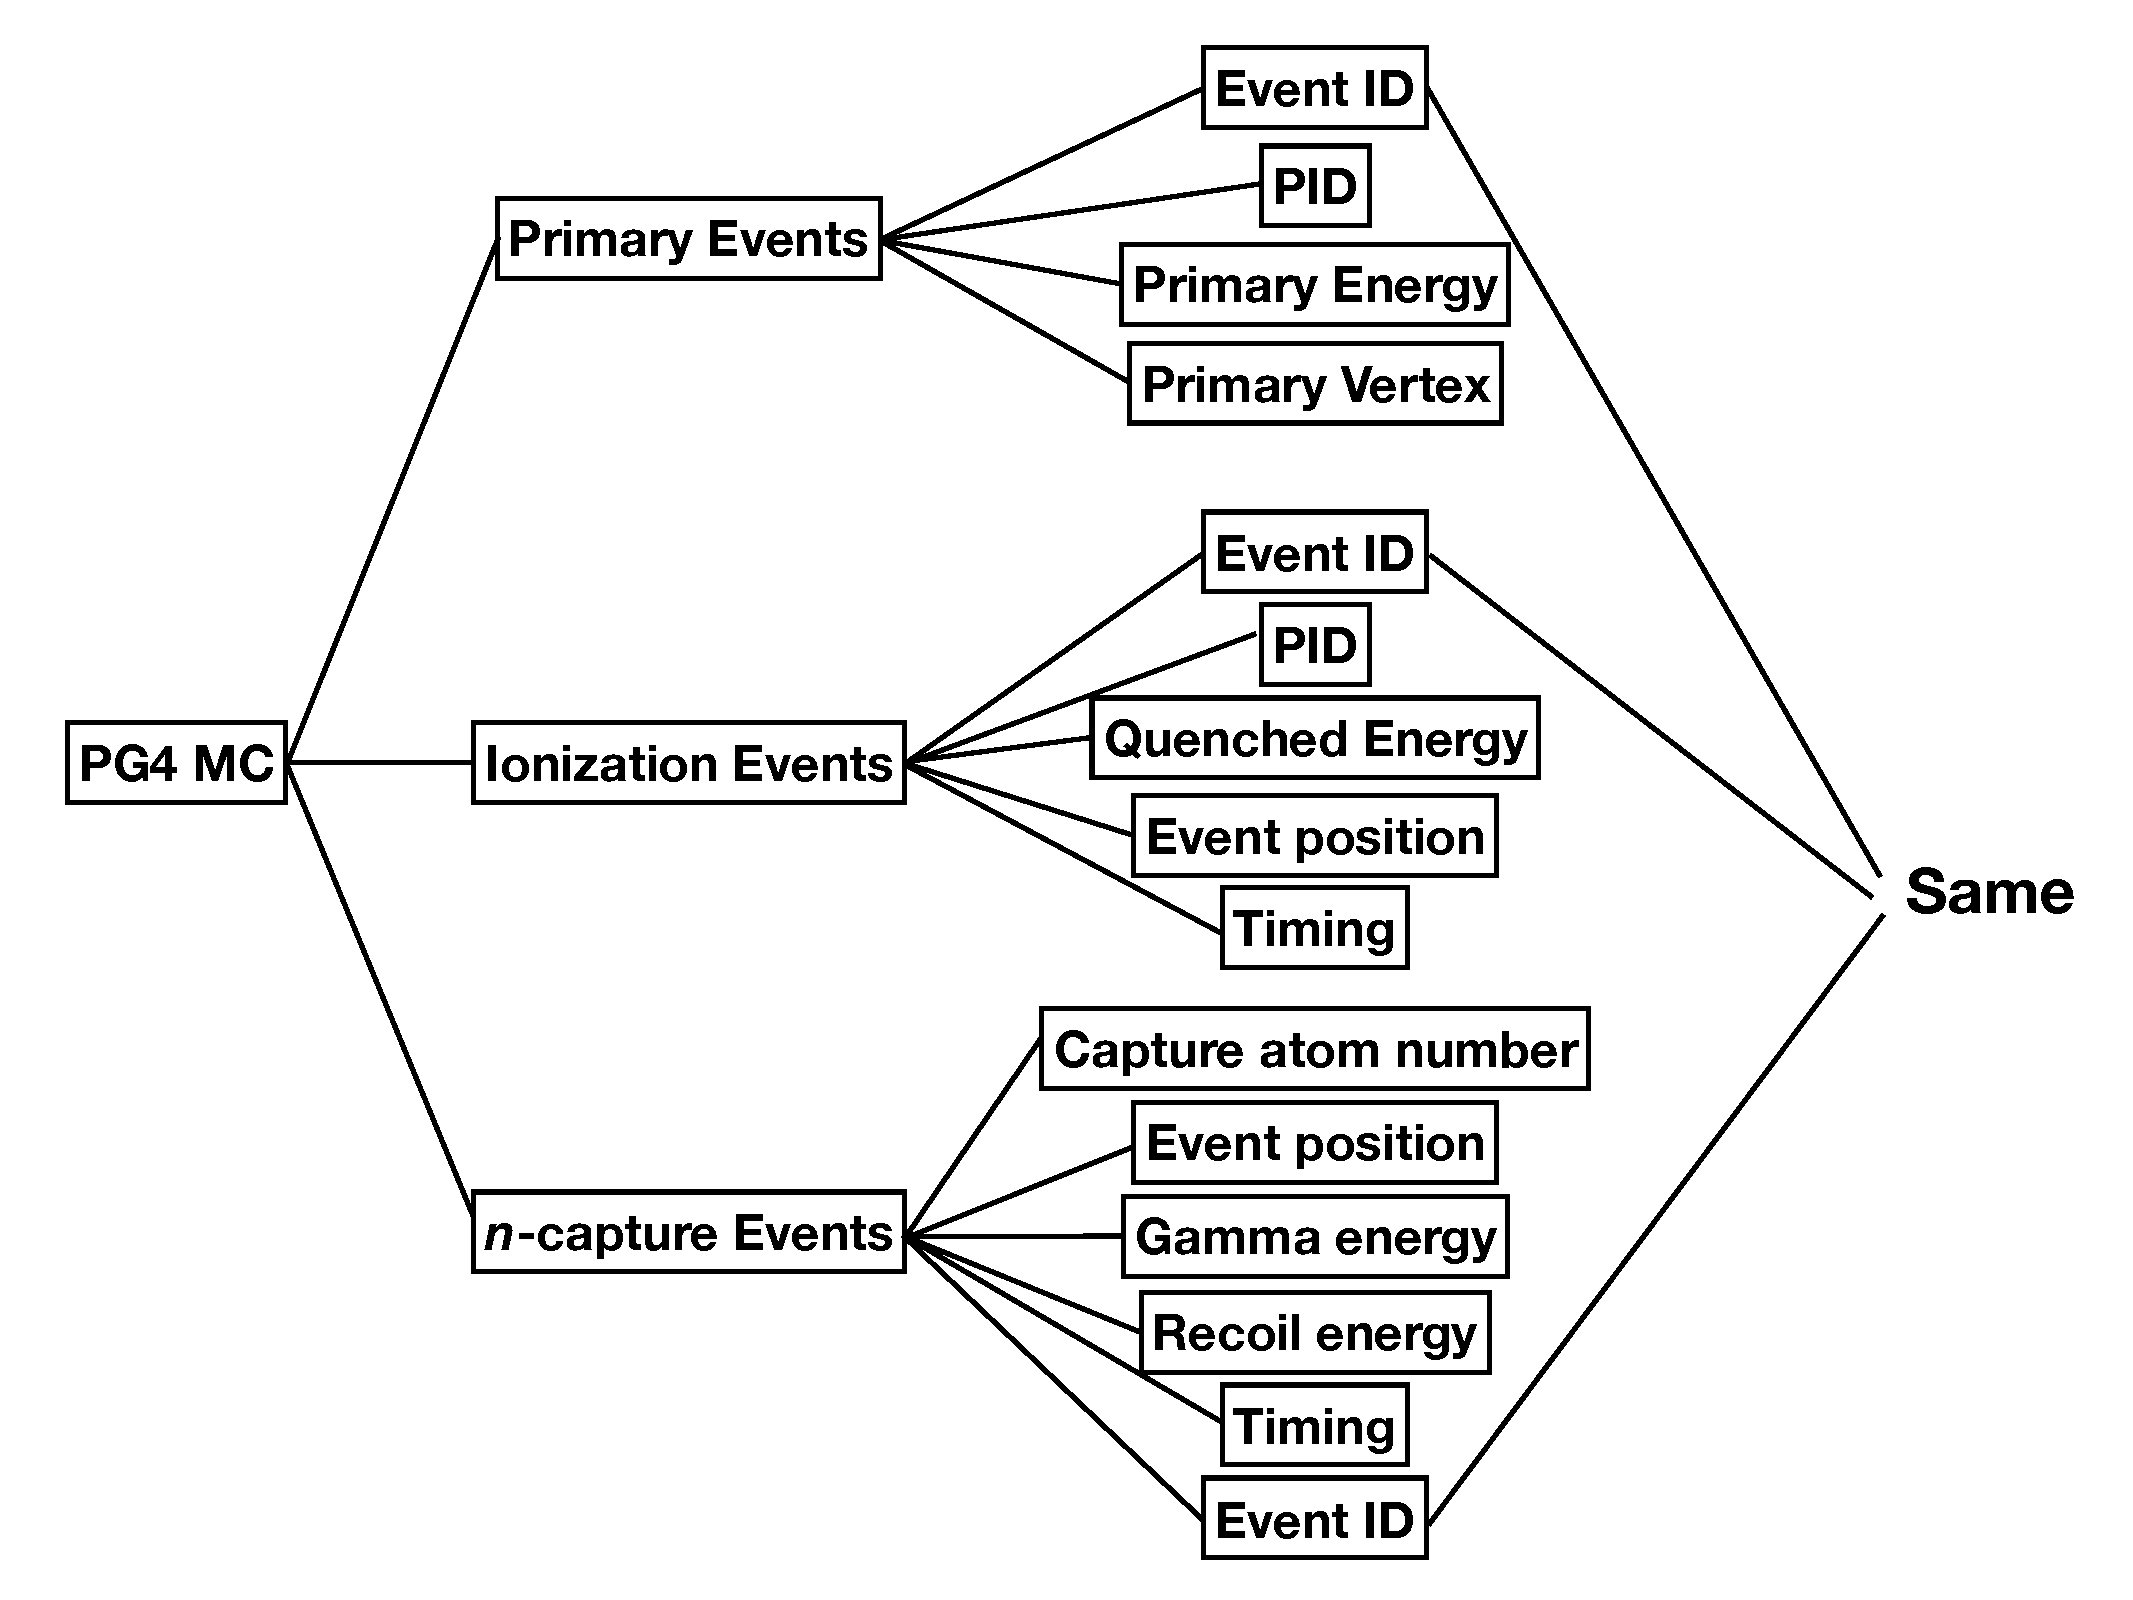
\includegraphics[width=0.8\textwidth]{Figures/MCStructure.pdf}\\
    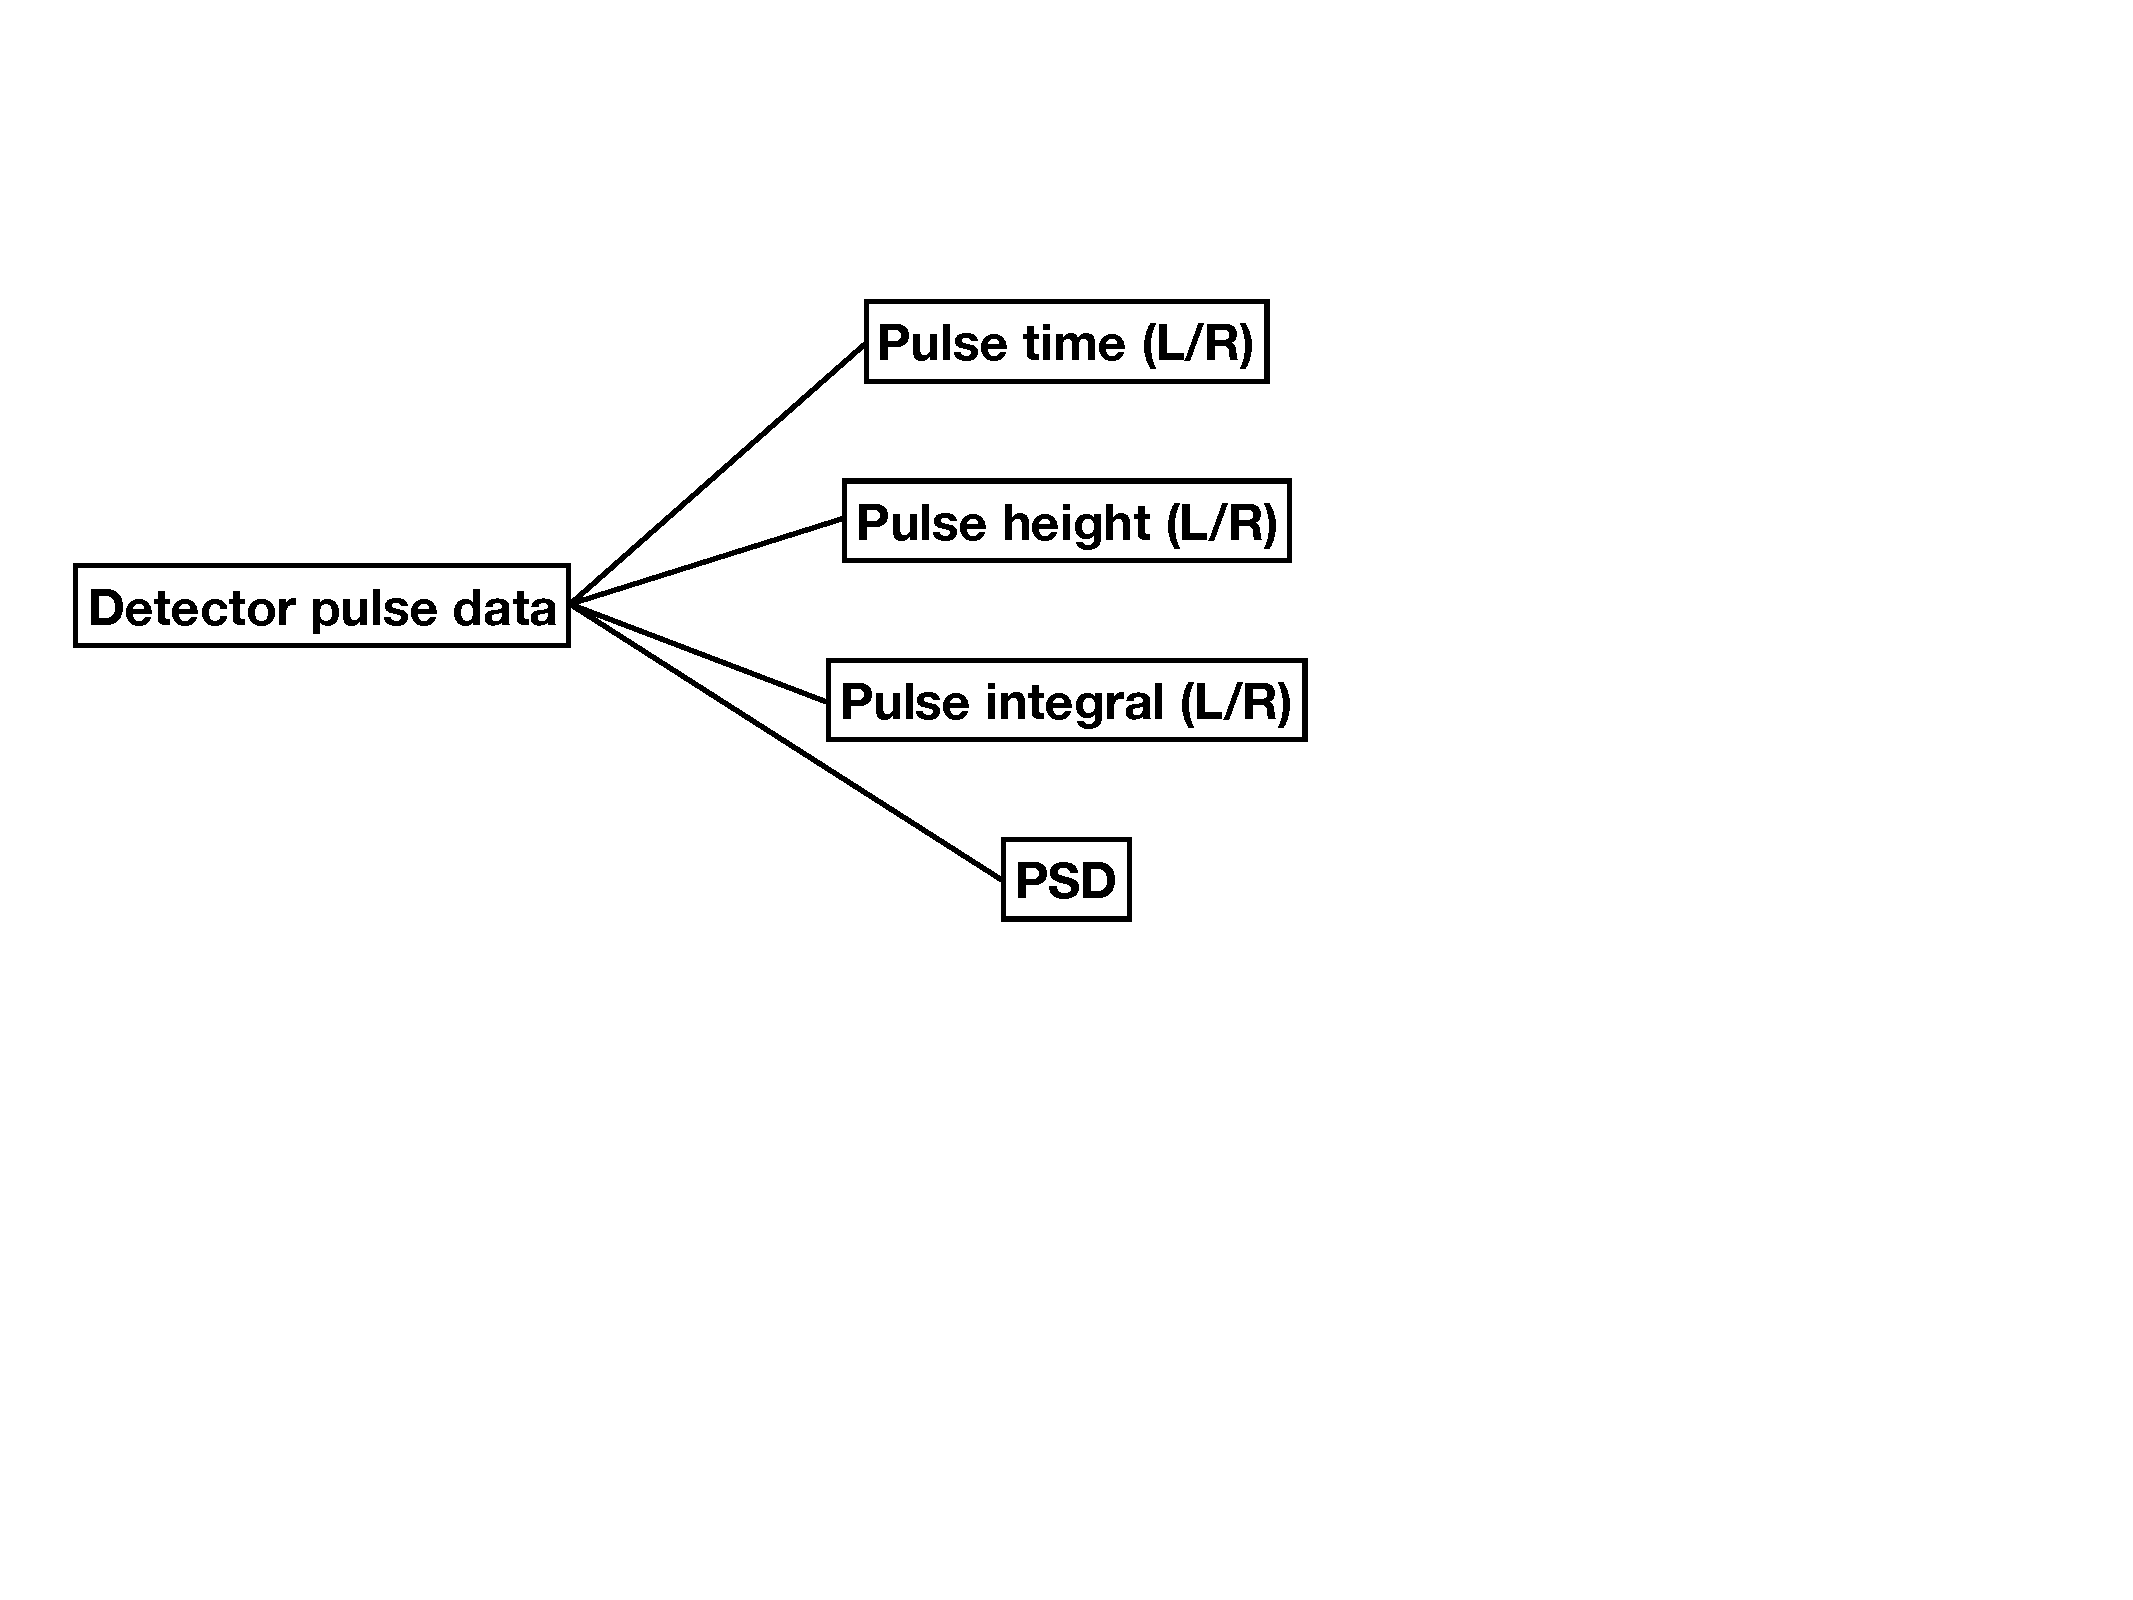
\includegraphics[width=0.5\textwidth]{Figures/PulseStructure.pdf}
	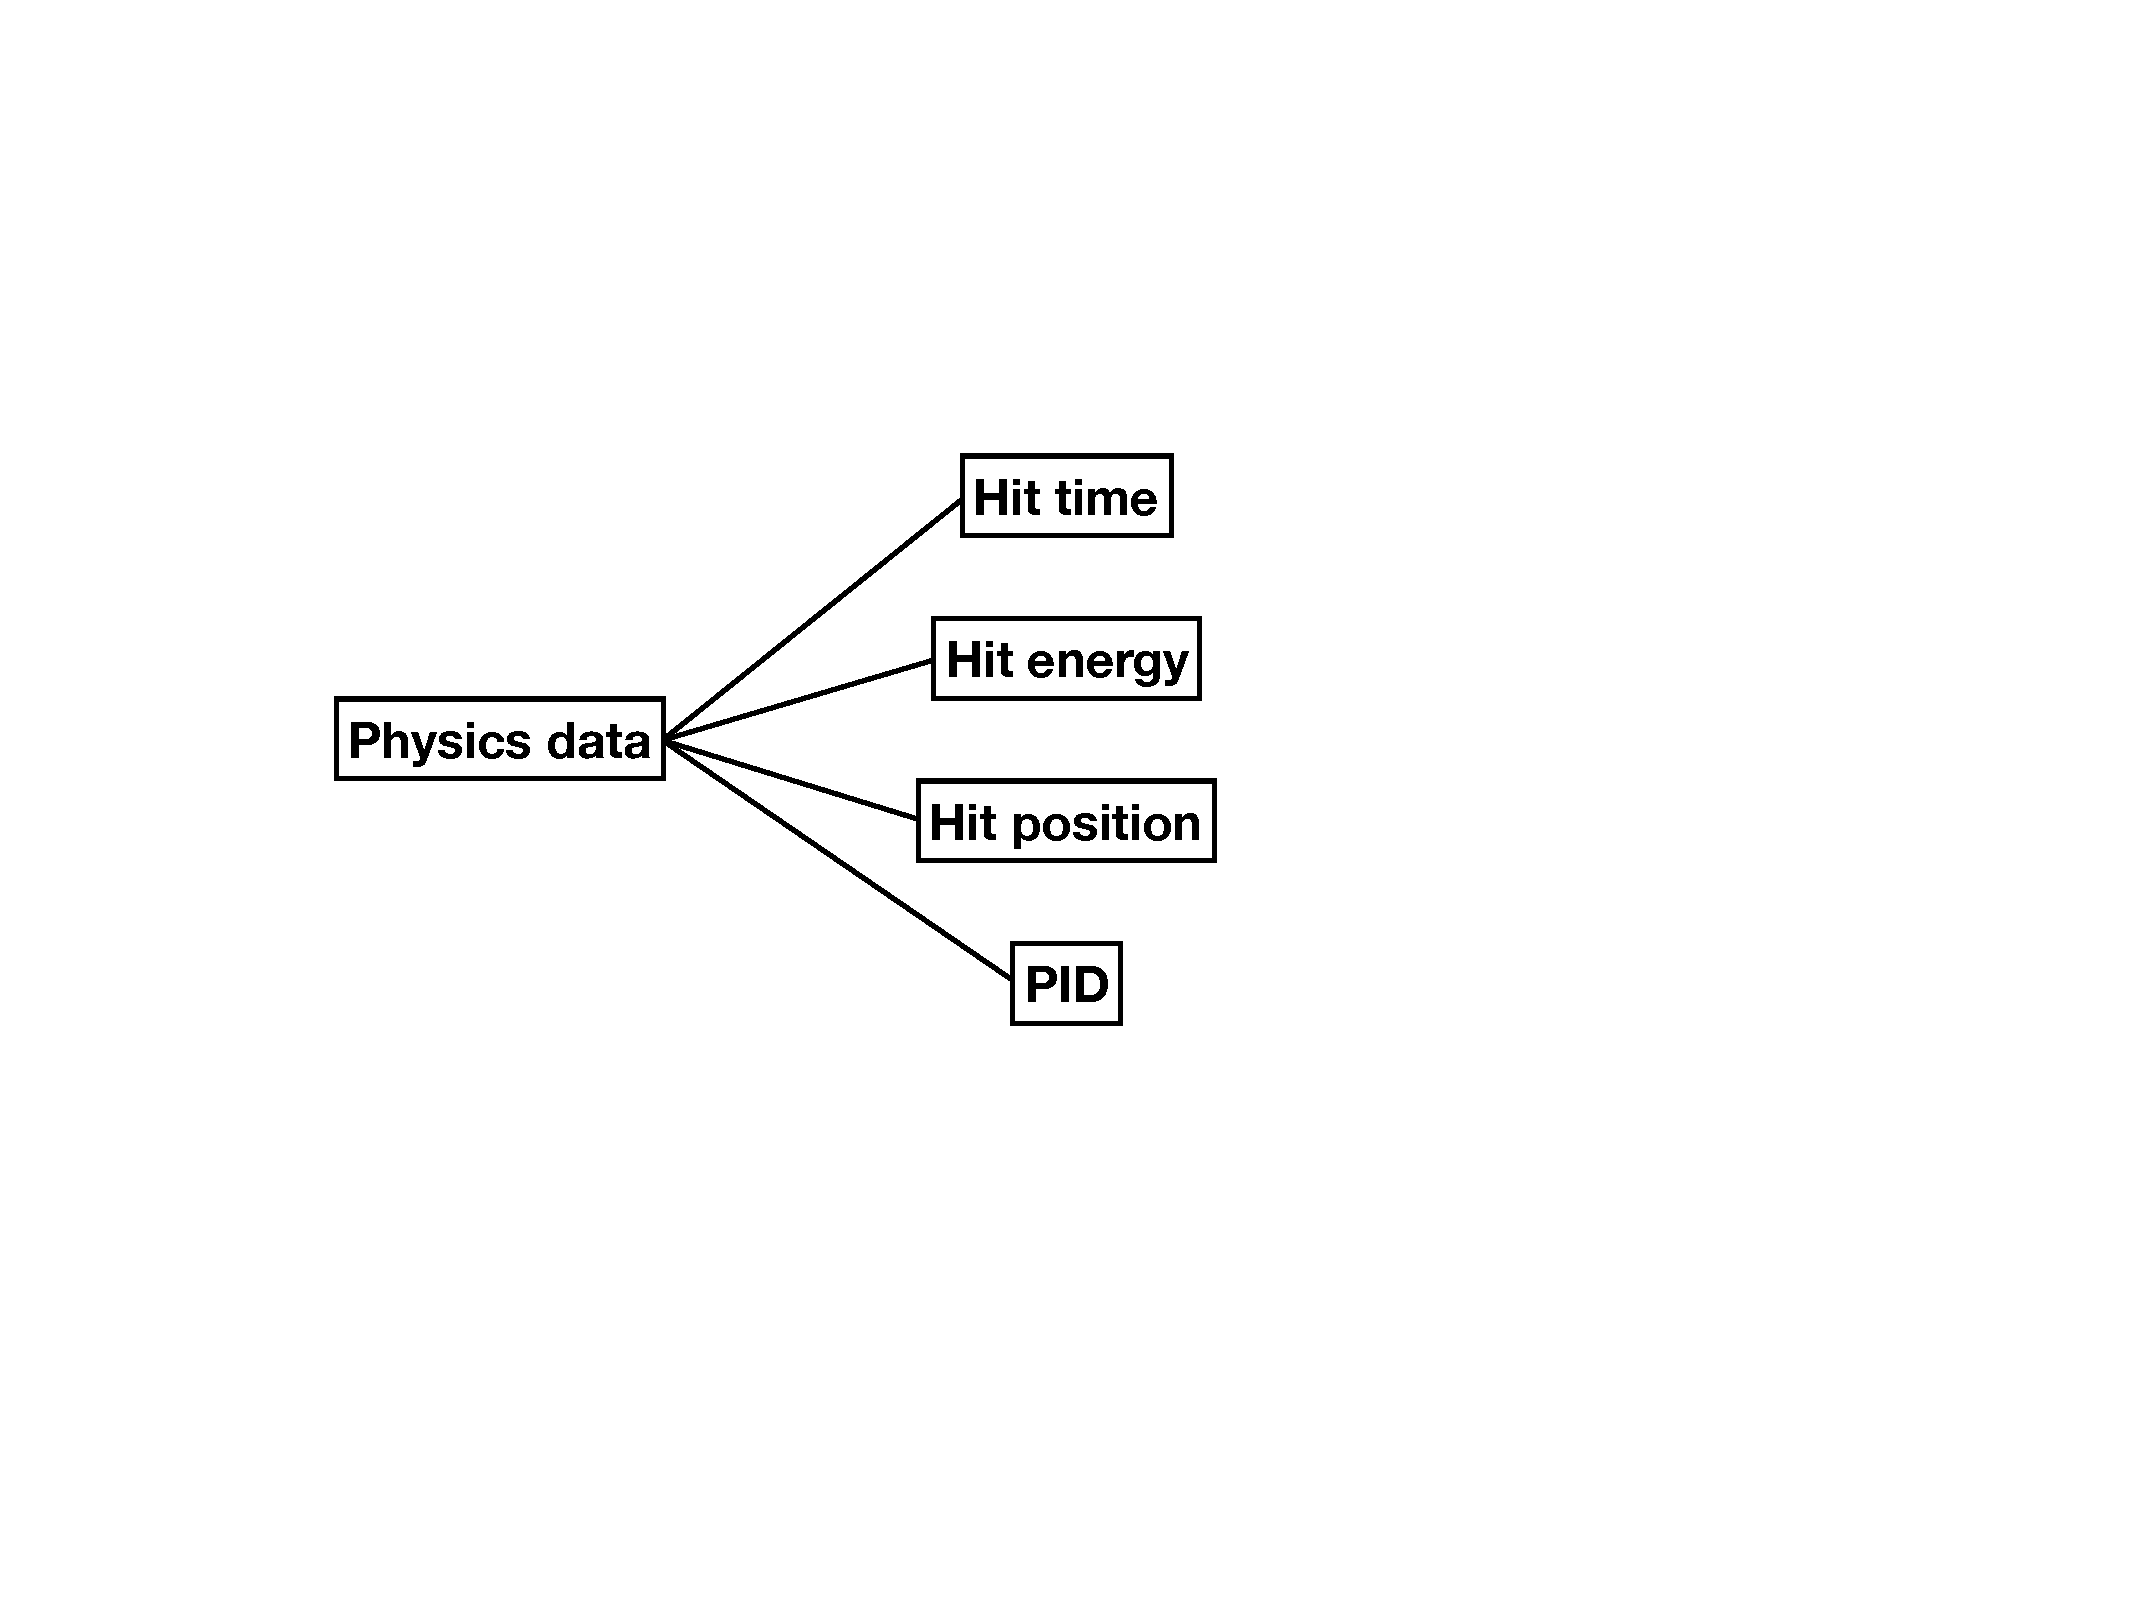
\includegraphics[width=0.4\textwidth]{Figures/PhysStructure.pdf}\\
	\caption[The data structure of MC simulation and PROSPECT data]{
	A schematic of the data structure of MC simulation and the actual PROSPECT data. 
	(Top) The structure of PG4 output, where the recorded categories share same event IDs.
	(Bottom left) The low level DAQ pulse data from unpacking the raw data. 
	(Bottom right) The high level physics data of the PROSPECT AD calibrated from the DAQ pulse data. 
    }
    \label{fig:MCstructure}
\end{figure}

The PG4 output is converted to simulated pulse and physics data through energy-ADC pulse conversion, which is a reversed conversion of the usual detector calibration, as shown in Figure~\ref{fig:MCconversion}.
PROSPECT's detector response information at different times, consisting the light response, DAQ gain setting, and PSD distributions, is saved in the PROSPECT calibration database. 
The MC energy deposition is converted to ADC channels based on this PROSPECT calibration database.
The calibration database saves ADC-energy calibration values with respect to time, and the template pulse shapes of different particles at each PMT channel.
Hence, the MC events can be converted to the simulated pulse data with PSD values, PMT pulses, and event time coincidences with time and position variations taken into consideration. 
The simulated pulse data can be calibrated to obtain simulated physics data, which is discussed in Chapter~\ref{Ch7}.
These procedures ensure precise detector response simulation even in the presence of non-uniformity and time-variation of the detector response.

\begin{figure}[h!]
    \centering
    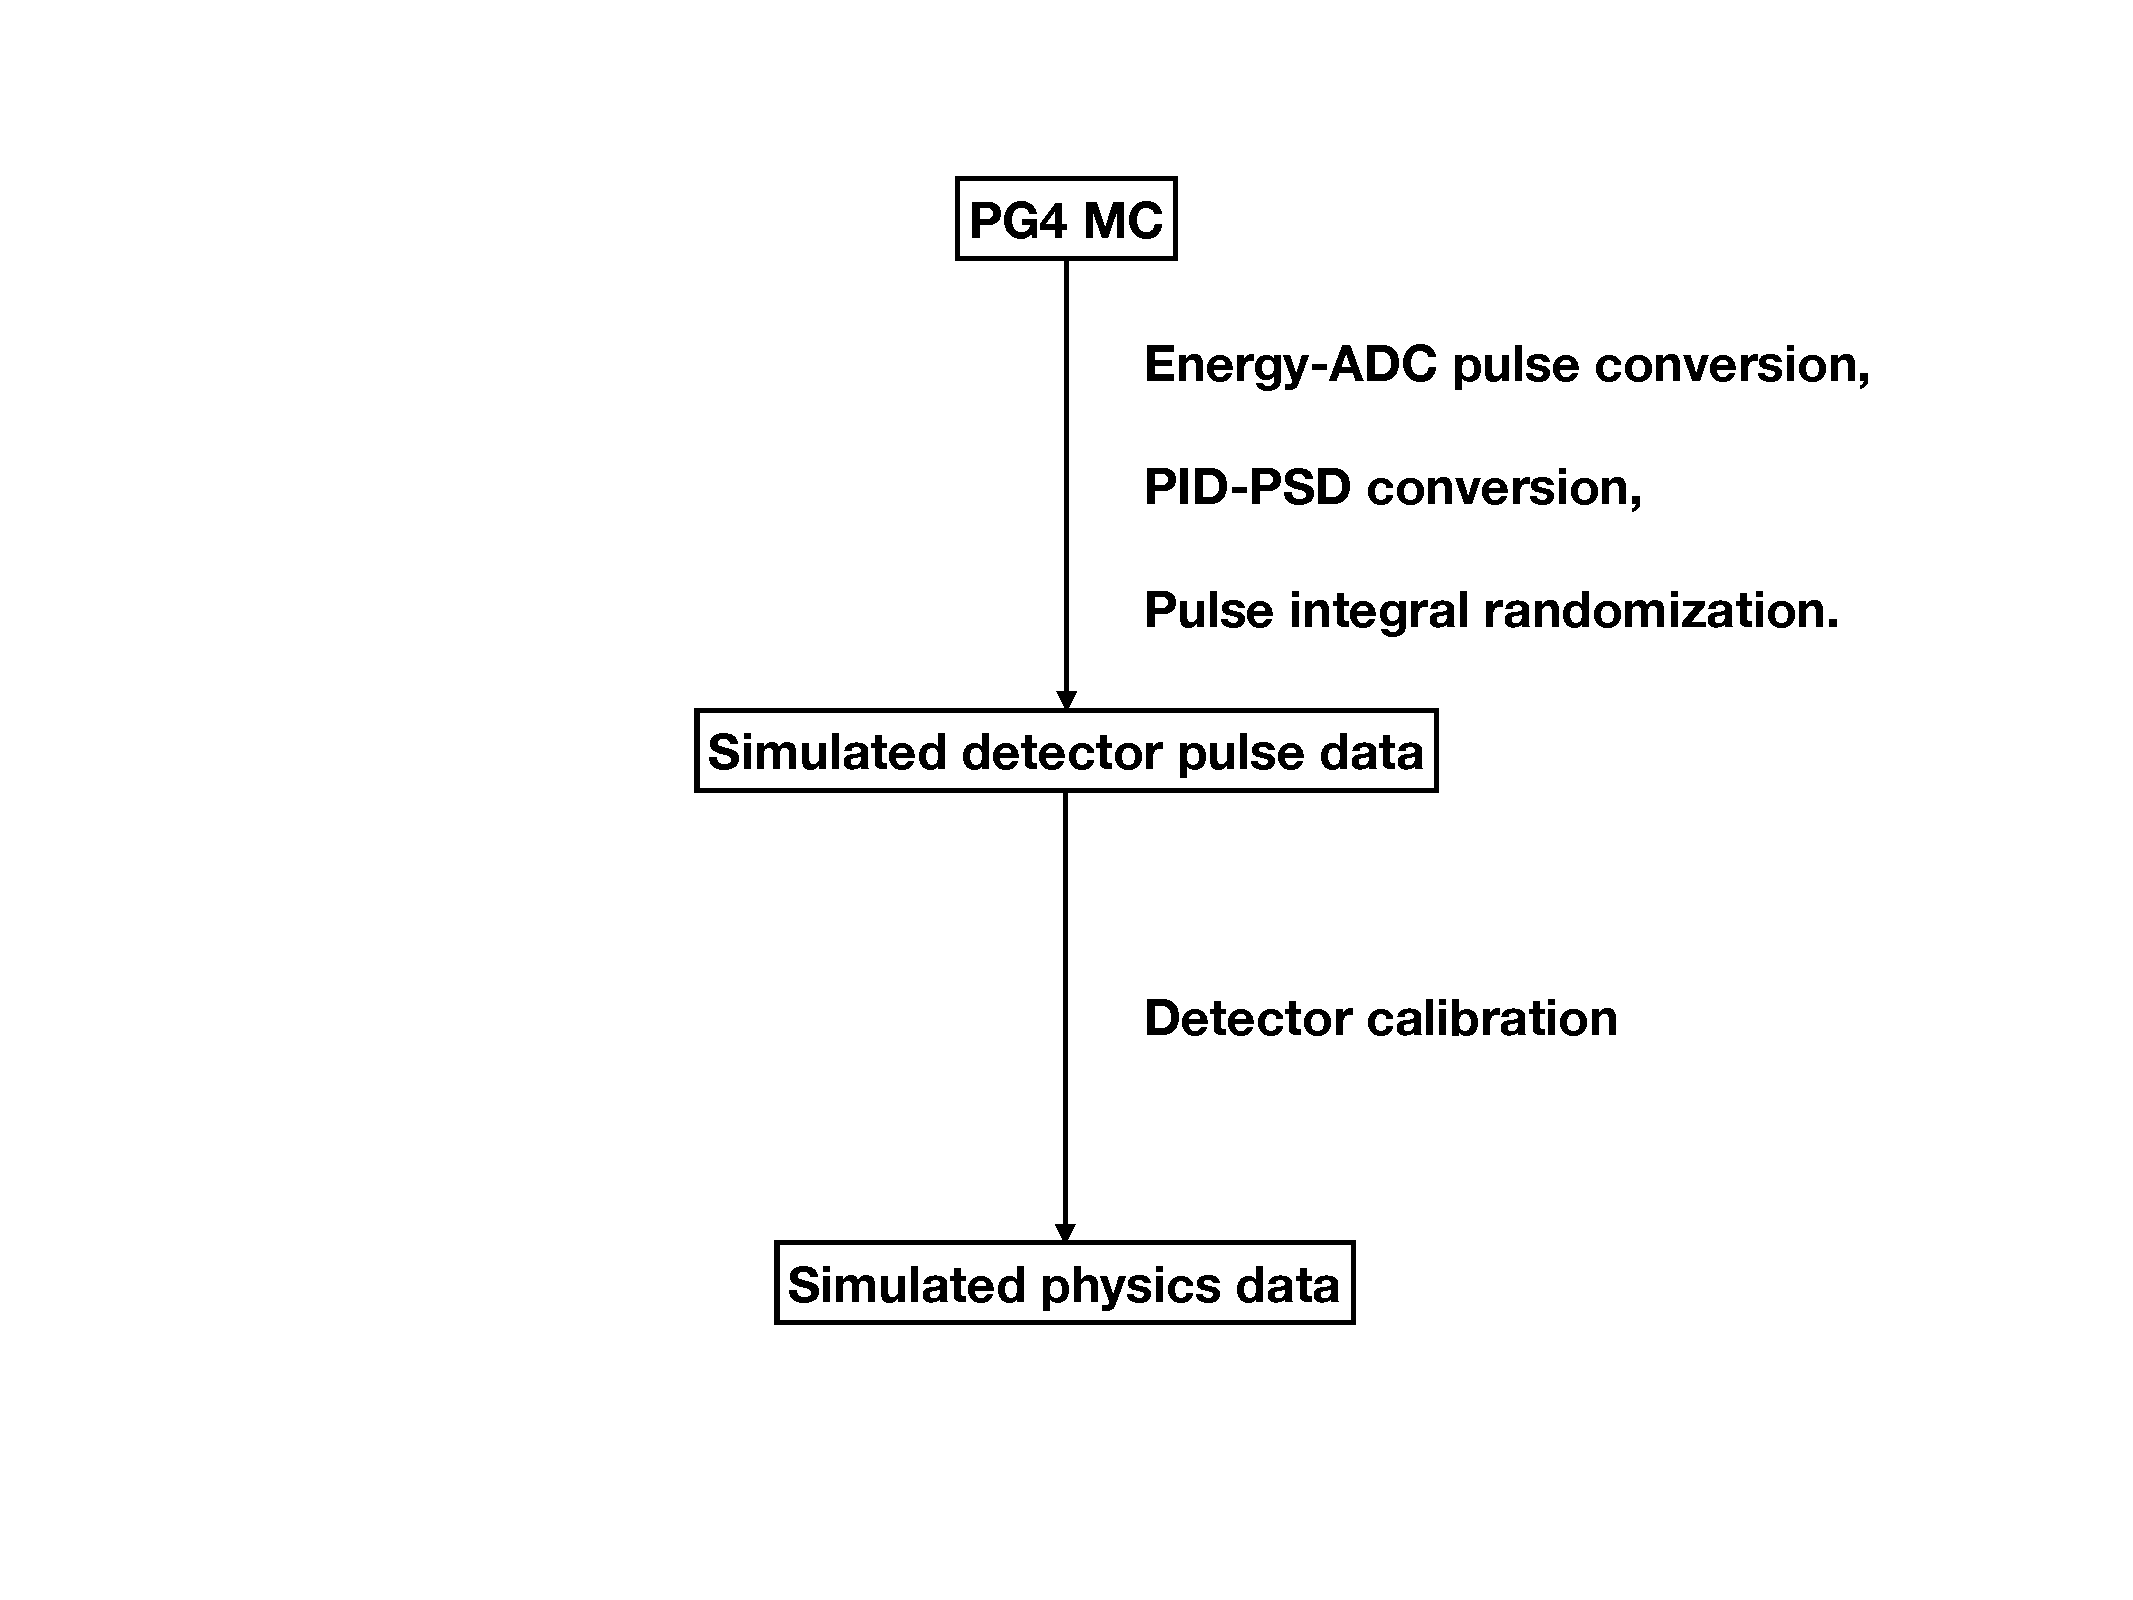
\includegraphics[width=0.9\textwidth]{Figures/MCconversion.pdf}\\
	\caption[Schematic of PG4 output conversion]{
	A schematic of PG4 output conversion procedures.
    }
    \label{fig:MCconversion}
\end{figure}